\chapter[Single CPU designs]{Single CPU designs}
\label{cha:singlecpu}

The purpose of this chapter is to describe in detail the single CPU design
support that is offered by \ee\ and by \rtd, highlighting the various
features available to the Altera developers.




\section[Single core Design Flow]
{Single core Design Flow}
\label{sec:singlecore-designflow}


The purpose of this section is to shortly describe the design flow
that must be used to develop a single core system using the tools
provided by Altera and by Evidence Srl. As it can be seen, the design
flow is equivalent to the current Altera design flow.

The first step of a Nios II single core system is the hardware
design. Every hardware design which is able to run the Altera HAL can
also run \ee. For example, the \const{standard},
\const{full_featured}, ... designs provided by Altera for the various
evaluation boards can be used as a starting point by the designer.

Once the hardware design has been defined, the designer can develop
the application software using Altera Nios II IDE (based on the Eclipse
Framework).

Using Nios II IDE the designer have to instantiate an Altera System
Library Project for each CPU in the system. The Altera System Library
contains the device drivers for the peripherals that are actually
connected to the CPU the library refers to. Please refer to the Altera
documentation on how to create a System Library.

After creating an Altera System Library for each CPU, the designer can
create an \rtd\ Project. The \rtd\ Project contains the application
that will run on the Nios II processor, and it is similar to the
``C/C++ Application'' project provided by Altera. As it will be
described later, the only difference with the Altera project is that
the configuration of the system is defined inside a text file which
follows the OSEK OIL specification \cite{OSEKOIL}. Figure
\ref{fig:altera-single-workflow} and
\ref{fig:evidence-single-workflow} graphically shows the difference
between the Altera and the Evidence approach: the Altera HAL approach
provides a C/C++ application project for each CPU, whereas \ee\
provides a \rtd\ project. \rtd\ Projects are described in Section
\ref{sec:niosII-basic-notions}, and in the \rtd\ Reference Manual.

Then, the designer compiles the application to create a set of
compiled files that are equivalent to the files generated by the
normal Altera Projects makefiles. As a result, the developer can debug
the application in the same way as all the other Altera HAL
applications.



%
\begin{figure}
\includegraphics[%
  width=1\columnwidth]{images/workflow_single_altera.eps}
\caption{\label{fig:altera-single-workflow}This Figure displays the
Altera approach to software development for single core Nios II
designs. Each Application is linked to a System Library which contains
the peripherals instantiated in SOPCBuilder for the CPU.}
\end{figure}

%
\begin{figure}
\includegraphics[%
  width=1\columnwidth]{images/workflow_single_evidence.eps}
\caption{\label{fig:evidence-single-workflow}This Figure displays the
Evidence Srl approach to software development for single core Nios II
designs. Each \rtd\ Project contains an OIL configuration file that
specifies the application and kernel configuration. The \rtd\ Project
is linked to a System Library which contains the peripherals
instantiated in SOPCBuilder for the CPU.}
\end{figure}






\section[System libraries]{Altera System libraries}

\ee\ uses the same System Libraries that are provided together with the
Altera HAL. When using the Altera System Libraries, developers have to
take care of the following issues:

\begin{itemize}
\item One System Library has to be created for each CPU in the system.

\item Separate stack space for exceptions should not be set inside the
  System Library properties. A similar feature can be obtained by
  setting a separate interrupt stack inside the OIL configuration
  file.

\item Custom linker scripts are supported with \ee.  Custom linker
  scripts can be specified inside the System Library project
  properties.
\end{itemize}


\section[Interrupts]{Using Interrupt handlers with \ee}

Users of the Altera HAL can continue to use the Altera provided
functions for interrupt handling. In particular,
\fn{alt_irq_register()} must be used to provide the registration of an
interrupt handler.  \fn{alt_irq_interruptible()} and
\fn{alt_irq_noninterrtptible()} must be used to handle interrupt
nesting. 

The Nios II \ee\ implementation considers all the interrupt handlers as
interrupts of category 2\index{ISR Category 2}. \ee\ correctly handles
interrupt nesting, performing appropriate checks at the end of the
last interrupt to implement task preemption. There is no support for
Interrupts of Category 1\index{ISR Category 1} in Nios II because of
the internal structure of the Nios II processor.

Among the options available on the Altera System Library Properties,
there is one named {\em Use a separate exception stack}\index{Separate
exception stack}, that can be used to allow interrupts and exceptions
stack to be allocated in separate memories. This feature is typically
used to move the interrupt stack in faster memories, such as on-chip
tightly coupled memories. When developing applications using \ee, the
separate stack as specified in the Altera System Library cannot be
used. A similar feature can be obtained with a multistack
configuration of \ee.



\section{The StartOS function}

To start the multiprogramming environment the designer have to call
the \fn{StartOS()}\index{StartOS} function inside \fn{main()} or
\fn{alt_main()}.

The \fn{StartOS()} primitive does the following actions:
\begin{enumerate}
\item It registers the interprocessor interrupt routine and
  initializes the Altera Mutex Peripheral.
\item It implements the startup barrier (only on a multicore system).
\item It calls StartupHook.
\item It activates autostart tasks and alarms.
\item It checks for preemption.
\item It returns to the caller.
\end{enumerate}

Please note that \fn{StartOS()} returns to the caller only when the
system have an idle time, that is, when all the task activations has
run.

The code literally after \fn{StartOS()} must correspond to background
activities that does not use \ee\ services.

If unsure of the code that have to be put after the call to
\fn{StartOS()}, use the following forever loop:

\begin{lstlisting}
for (;;);
\end{lstlisting}





\section{Altera Nios II IDE tips and tricks}

This is a list of the preferences of the Altera Nios II IDE that needs
a modification:

\begin{description}
\item[Allow multiple active runs.]  This option can be found in
  ``window/preferences/nios2/ allow multiple active runs''. You need to
  set this option to be able to debug multicore systems (see
  Figure \ref{fig:Nios2-preference})

\item[Build if required] This option can be found in
  ``window/preferences/rundebug/launching/build if required''. This
  option can be used disable the application automatic build (see
  Figure \ref{fig:Nios2-buildifrequired}. Since building a
  multicore system may require a lot of time, this options
  waiting time when avoids automatic building when the user has to
  start different debug sessions without need of recompiling the
  system.
\end{description}

\begin{figure}
  \begin{center}
    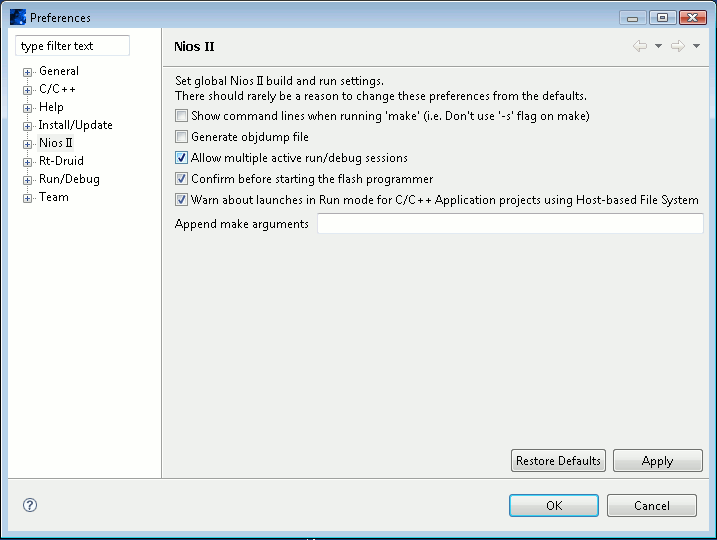
\includegraphics[width=7cm, bb=0 0 717 540]{images/Nios2_preferences.png}
  \end{center}
  \caption{Nios 2 IDE preference window. The ``Allow multiple runs'' checkbox must be checked.}
  \label{fig:Nios2-preference} 
\end{figure}

\begin{figure}
  \begin{center}
    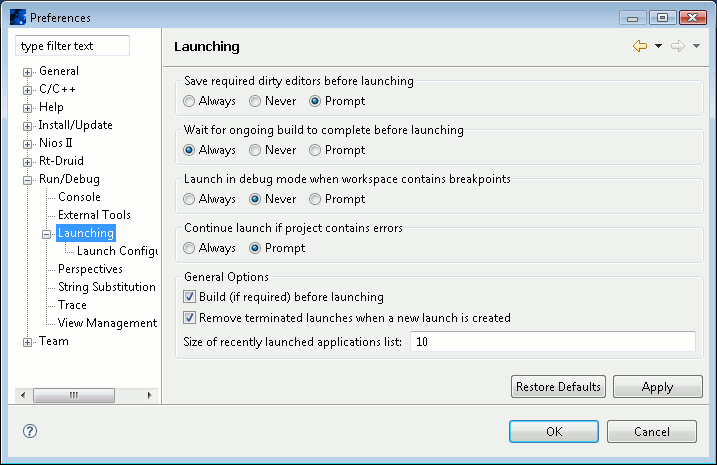
\includegraphics[width=7cm, bb=0 0 717 465]{images/Nios2_buildifrequired.png}
  \end{center}
  \caption{Nios 2 IDE preference Run/Debug window. Consider unchecking the ``Build if Required'' checkbox.}
  \label{fig:Nios2-buildifrequired} 
\end{figure}




\section[Altera Device Drivers]{Usage of the Altera HAL device drivers with \ee}

\ee\ currently does not provide any customized versions of the Altera
HAL device drivers.

In general, the Altera HAL device drivers have to be used with care in
multitask application developed with \ee, because these
device drivers are designed for a single task environment.

In particular, some care have to be taken avoiding that more than one
task calls a device driver set of primitives concurrently. There are
two possibilities:

\begin{itemize}
\item Allocate a dedicated task that is the only one that uses a given
      device driver primitive (for example, if a CPU has a JTAG UART,
      the user should allocate a single task that is responsible for
      the standard input/standard output operations on that
      peripheral).

\item Allow different tasks to use the primitives in a mutual
      exclusive way. In that case, mutual exclusion can be obtained
      using a Resource dedicated to the purpose, and using GetResource
      and ReleaseResource primitives to sequentialize the accesses to
      the shared resource.
\end{itemize}

In general, all the file system primitives that are potentially
blocking on a system are implemented with a busy wait within the
HAL. For that reason, use these primitives in non-blocking mode. Future
versions of \ee\ will include a customization of the Altera HAL drivers
to allow file system primitives to become blocking primitives.


